\documentclass[a4paper]{article}
\usepackage{a4wide,amssymb,epsfig,latexsym,multicol,array,hhline,fancyhdr}
\usepackage[utf8]{vntex, inputenc}
\usepackage[english]{babel}
\usepackage{amsmath}
\usepackage{lastpage}
\usepackage[lined,boxed,commentsnumbered]{algorithm2e}
\usepackage{enumerate}
\usepackage{color}
\usepackage{graphicx}							% Standard graphics package
\usepackage{array}
\usepackage{tabularx, caption}
\usepackage{multirow}
\usepackage{multicol}
\usepackage{rotating}
\usepackage{graphics}
\usepackage{geometry}
\usepackage{setspace}
\usepackage{epsfig}
\usepackage{tikz}
\usetikzlibrary{arrows,snakes,backgrounds}
\usepackage{hyperref}
\usepackage{indentfirst}
\usepackage{float}
\hypersetup{urlcolor=blue,linkcolor=black,citecolor=black,colorlinks=true}
%\usepackage{pstcol} 								% PSTricks with the standard color package

\newtheorem{theorem}{{\bf Theorem}}
\newtheorem{property}{{\bf Property}}
\newtheorem{proposition}{{\bf Proposition}}
\newtheorem{corollary}[proposition]{{\bf Corollary}}
\newtheorem{lemma}[proposition]{{\bf Lemma}}

\AtBeginDocument{\renewcommand*\contentsname{Contents}}
\AtBeginDocument{\renewcommand*\refname{References}}
%\usepackage{fancyhdr}
\setlength{\headheight}{40pt}
\pagestyle{fancy}
\fancyhead{} % clear all header fields
\fancyhead[L]{
  \begin{tabular}{rl}
    \begin{picture}(25,15)(0,0)
    \put(0,-8){
\includegraphics[width=8mm, height=8mm]{hcmut.png}}
    %\put(0,-8){\epsfig{width=10mm,figure=hcmut.eps}}
    \end{picture}
	%
\includegraphics[width=8mm, height=8mm]{hcmut.png} & %
    \begin{tabular}{l}
      \textbf{\bf \ttfamily University of Technology, Ho Chi Minh City}\\
      \textbf{\bf \ttfamily Faculty of Computer Science and Engineering}
    \end{tabular}
  \end{tabular}
}
\fancyhead[R]{
	\begin{tabular}{l}
		\tiny \bf \\
		\tiny \bf
	\end{tabular}  }
\fancyfoot{} % clear all footer fields
\fancyfoot[L]{\scriptsize \ttfamily Assignment for Mathematical Modeling\textendash{}Academic year 2020\textendash{}2021}
\fancyfoot[R]{\scriptsize \ttfamily Page {\thepage}/\pageref{LastPage}}
\renewcommand{\headrulewidth}{0.3pt}
\renewcommand{\footrulewidth}{0.3pt}


%%%
\setcounter{secnumdepth}{4}
\setcounter{tocdepth}{3}
\makeatletter
\newcounter{subsubsubsection}[subsubsection]
\renewcommand\thesubsubsubsection{\thesubsubsection.\@alph\c@subsubsubsection}
\newcommand\subsubsubsection{\@startsection{subsubsubsection}{4}{\z@}%
                                     {-3.25ex\@plus-1ex \@minus-.2ex}%
                                     {1.5ex \@plus.2ex}%
                                     {\normalfont\normalsize\bfseries}}
\newcommand*\l@subsubsubsection{\@dottedtocline{3}{10.0em}{4.1em}}
\newcommand*{\subsubsubsectionmark}[1]{}
\makeatother


\begin{document}

\begin{titlepage}
  \begin{center}
    VIETNAM NATIONAL UNIVERSITY, HO CHI MINH CITY \\
    UNIVERSITY OF TECHNOLOGY \\
    FACULTY OF COMPUTER SCIENCE AND ENGINEERING
  \end{center}

  \vspace{1cm}

  \begin{figure}[h!]
    \begin{center}
      
\includegraphics[width=3cm]{hcmut.png}
    \end{center}
  \end{figure}

  \vspace{1cm}


  \begin{center}
    \begin{tabular}{c}
      \multicolumn{1}{l}{\textbf{{\Large MATHEMATICAL MODELING  (CO2011)}}}               \\
      {}                                                                                  \\
      \hline
      \\
      \multicolumn{1}{l}{\textbf{{\Large Assignment (Semester 201, Duration: 06 weeks)}}} \\
      \\
      \textbf{{\Huge Dynamical systems in forecasting}}                                   \\
      \\
      \textbf{{\Huge Greenhouse Micro-climate}}                                           \\
      \\
      \hline
    \end{tabular}
  \end{center}

  \vspace{3cm}

  \begin{table}[h]
    \begin{tabular}{rrl}
      \hspace{5 cm} & Advisor: & Nguyễn Tiến Thịnh \\
                    &          & Nguyễn An Khương  \\
                    & TA:      & Trần Trung Hiếu   \\
    \end{tabular}
  \end{table}

  \begin{center}
    {\footnotesize HO CHI MINH CITY, DECEMBER 2020}
  \end{center}
\end{titlepage}


%\thispagestyle{empty}

\newpage
\tableofcontents
\newpage


%%%%%%%%%%%%%%%%%%%%%%%%%%%%%%%%%
\section{Member list \& Workload}

\begin{center}
  \begin{tabular}{|c|c|c|l|c|}
    \hline
    \textbf{No.}       & \textbf{Fullname}                      & \textbf{Student ID}      & \textbf{Problems}                             & \textbf{Percentage of work} \\
    \hline
    %%%%%Student 1%%%%%%%%%%
    \multirow{3}{*}{1} & \multirow{3}{*}{Lưu Nguyễn Hoàng Minh} & \multirow{3}{*}{1952845} & \textendash{} Relation \& Counting: 1, 2, 3   & \multirow{3}{*}{20\%}       \\
                       &                                        &                          & Bonus: 1, 2, 3.                               &                             \\
                       &                                        &                          & \textendash{} Probability: 1, 2, 3.           &                             \\
    \hline
    %%%%%Student 2%%%%%%%%%%%
    \multirow{3}{*}{2} & \multirow{3}{*}{Vũ Anh Nhi}            & \multirow{3}{*}{1952380} & \textendash{} Relation \& Counting: 4, 5, 6   & \multirow{3}{*}{20\%}       \\
                       &                                        &                          & Bonus: 4, 5, 6.                               &                             \\
                       &                                        &                          & \textendash{} Graph: 1, 2, 3, Bonus: 1, 2, 3. &                             \\
    \hline
    %%%%%Student 3%%%%%%%%%%%
    \multirow{3}{*}{2} & \multirow{3}{*}{Nguyễn Phú Nghĩa}      & \multirow{3}{*}{1952355} & \textendash{} Relation \& Counting: 4, 5, 6   & \multirow{3}{*}{20\%}       \\
                       &                                        &                          & Bonus: 4, 5, 6.                               &                             \\
                       &                                        &                          & \textendash{} Graph: 1, 2, 3, Bonus: 1, 2, 3. &                             \\
    \hline
    %%%%%Student 4%%%%%%%%%%%
    \multirow{3}{*}{2} & \multirow{3}{*}{Nguyễn Chính Khôi}     & \multirow{3}{*}{1952793} & \textendash{} Relation \& Counting: 4, 5, 6   & \multirow{3}{*}{20\%}       \\
                       &                                        &                          & Bonus: 4, 5, 6.                               &                             \\
                       &                                        &                          & \textendash{} Graph: 1, 2, 3, Bonus: 1, 2, 3. &                             \\
    \hline
    %%%%%Student 5%%%%%%%%%%%
    \multirow{3}{*}{2} & \multirow{3}{*}{Nguyễn Hoàng}          & \multirow{3}{*}{1952255} & \textendash{} Relation \& Counting: 4, 5, 6   & \multirow{3}{*}{20\%}       \\
                       &                                        &                          & Bonus: 4, 5, 6.                               &                             \\
                       &                                        &                          & \textendash{} Graph: 1, 2, 3, Bonus: 1, 2, 3. &                             \\
    \hline
  \end{tabular}
\end{center}


%%%%%%%%%%%%%%%%%%%%%%%%%%%%%%%%%
\section{Exercise 1}
\subsection{(a)}
A dynamical system is any system that evolves or changes with respect to time according to some rules.
A state space, also called the phase space, is a model used within dynamical systems to capture these changes.
For investigating dynamical systems, it is necessary to specify some characteristics that provide a subdivision into special classes of dynamical systems.

Dynamical systems are often classified as continuous or discrete.
Continuous systems (also called flows) are given by differential equations.
In such systems, the time intervals between measurements are negligibly small, making changes appear as one long continuum.
Then there are discrete systems (also called maps), which are specified by difference equations.

Another important characteristic of a dynamical system is whether it is time dependent or not.
For time-dependent systems, the function that specifies \(\dot{x}\) or \(\Delta{x_n}\) depends on the time itself, whereas in time-independent systems, this function does not change.

For the analysis, it is important whether a dynamical system is linear or not.
Linear dynamical systems are simple to analyze, unlike non-linear systems, which typically have intricate dynamical behavior.

A general dynamical system contains 2 elements: the initial state and a function or functions describing the next state.
We can choose any point in the state space to be the origin, then depending on the requirements, our functions can be differential or difference.
\begin{equation}
  \begin{cases}
    a_0           & = C \\
    \frac{da}{dt} & = f
  \end{cases}
\end{equation}
or
\begin{equation}
  \begin{cases}
    a_0       & = C       \\
    a_{n + 1} & = a_n + X
  \end{cases}
\end{equation}
with \(f\) is an arbitrary function or functions, \(C\) and \(X\) are arbitrary constants.

In this assignment, we are required to design first-order differential systems to predict the climate inside an arbitrary greenhouse.
% TODO

\subsection{(b)}
% TODO

\subsection{(c)}
% TODO

\subsection{(d)}
% TODO

\subsection{(e)}
% TODO


%%%%%%%%%%%%%%%%%%%%%%%%%%%%%%%%%
\section{Exercise 2}
\subsection{a)}
\subsubsubsection{Chapter 2}
\begin{figure}[H]
  \centering
  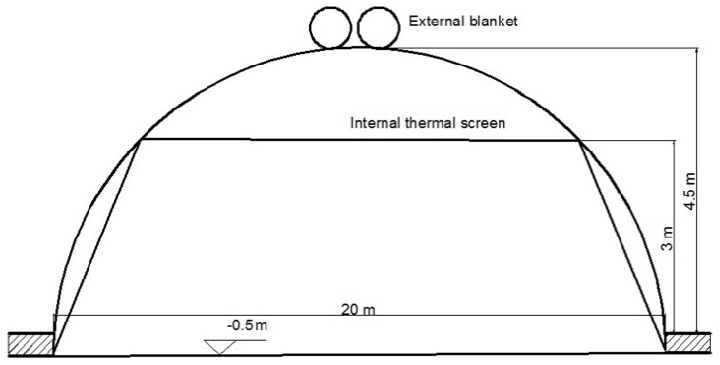
\includegraphics[width=\textwidth]{thrscr.png}
  \caption{The CO2 flow inside and outside a greenhouse.}\label{fig:thrscr}
\end{figure}
\begin{figure}[H]
  \centering
  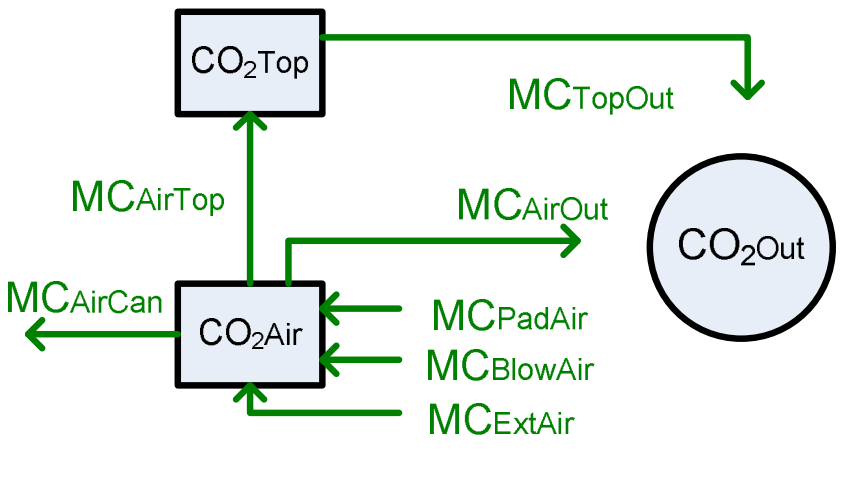
\includegraphics[width=\textwidth]{CO2}
  \caption{The CO2 flow inside and outside a greenhouse.}\label{fig:CO2}
\end{figure}

% TODO


\subsection{b)}
% TODO


%%%%%%%%%%%%%%%%%%%%%%%%%%%%%%%%%
\section{Exercise 3}
% TODO


%%%%%%%%%%%%%%%%%%%%%%%%%%%%%%%%%
\section{Exercise 4}
\subsection{a)}
% TODO

\subsection{b)}
% TODO


%%%%%%%%%%%%%%%%%%%%%%%%%%%%%%%%%
\section{Exercise 5}
% TODO
\begin{figure}[H]
  \centering
  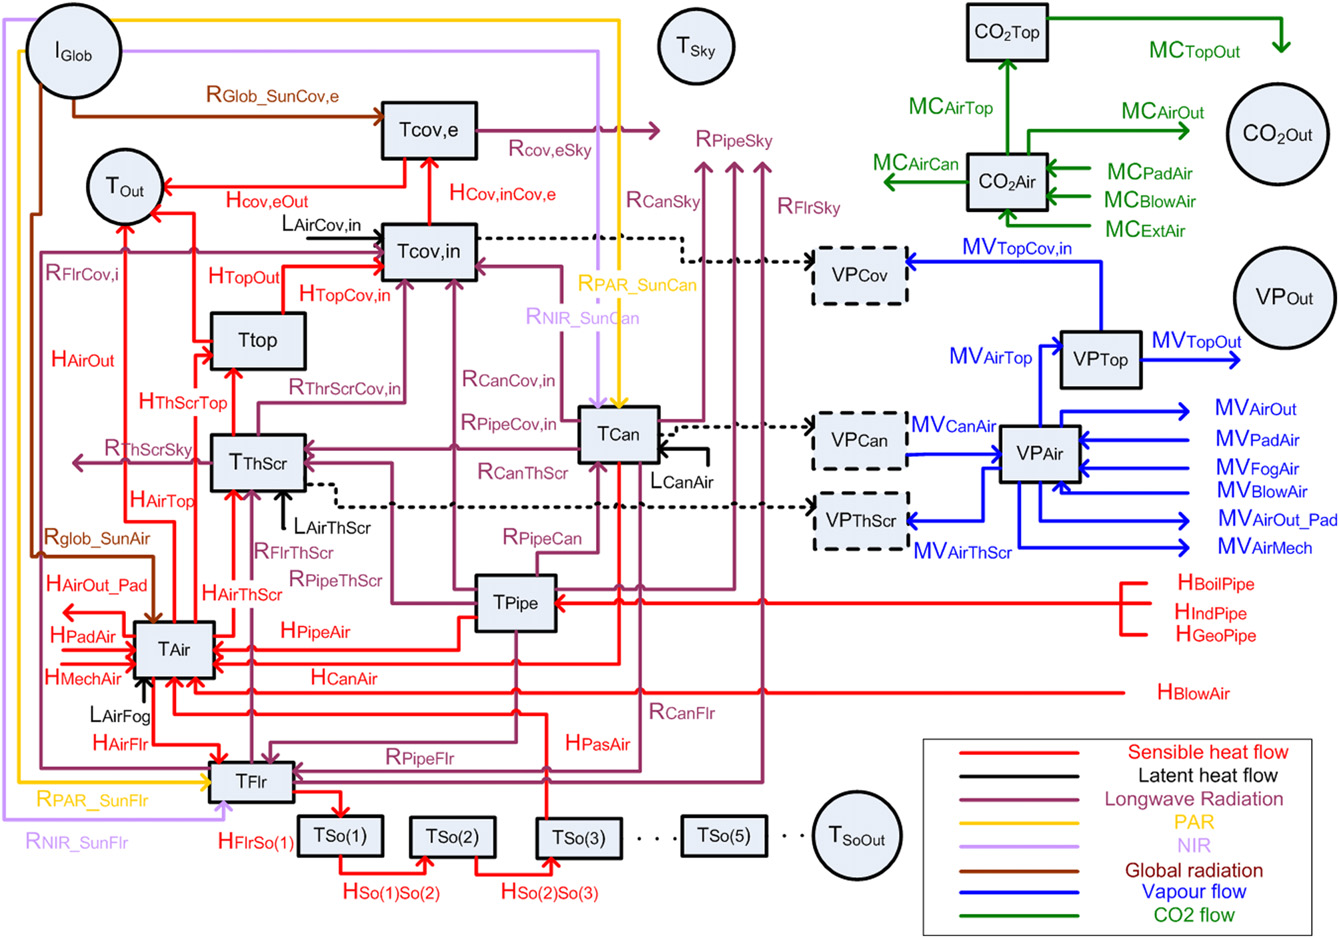
\includegraphics[width=\textwidth]{overview}
  \caption{Overview of the greenhouse model}\label{fig:overview}
\end{figure}

In this section, a dynamical system representing the vapor pressure in the greenhouse will be addressed.
The model was based on the following assumption:
1) the greenhouse air is considered to be a ``perfectly stirred tank'', meaning that there are no spatial differences in temperature, vapor pressure and the \(CO_2\) concentration; thus all the model fluxes are described per square metre of greenhouse floor;
2) to describe the effect of the thermal screen on the indoor climate, the greenhouse air was divided into two compartments: one below and one above the thermal screen.

From figure~\ref{fig:overview}, the vapor pressure of the greenhouse air \(VP_{Air}\) and the top compartment \(VP_{Top}\) are described by: \\
\begin{equation}
  \begin{split}
    cap_{VP_{Air}}\dot{VP_{Air}} = &\;MV_{CanAir} + MV_{PadAir} + MV_{FogAir} + MV_{BlowAir} \\
    & -MV_{AirThScr} - MV_{AirTop} - MV_{AirOut} - MV_{AirOut\_Pad} \\
    & -MV_{AirMech} ~~~~~~~~~~~~~~~~~~~~~~~~~~~~~~~~~~~~~~~~~ [kg\;m^{-2}\;s^{-1}]
  \end{split}
\end{equation}
\begin{equation}
  cap_{VP_{Top}}\dot{VP_{Top}} = MV_{AirTop} - MV_{TopCov,in} - MV_{TopOut} ~~~~~~~~ [kg\;m^{-2}\;s^{-1}]
\end{equation}
The notations \(cap_X\), \(VP_X\), \(\dot{VP_X}\) and \(MV_{XY}\) are respectively the capacity to store vapor pressure in X (\(kg\;m^3\;J^{-1}\)),
the vapor pressure in X (\(Pa\)), the rate of change of vapor pressure in X (\(Pa\;s^{-1}\)), and the net vapor flux from X to Y (\(kg\;m^{-2}\;s^{-1}\)),
where \(Air\) and \(Top\) denote the lower and upper compartments, \(Can\) represents the canopy, \(Pad\) represents the pad system, \(Fog\) represents the fogging system,
\(Blow\) represents the direct air heater, \(ThScr\) represents the thermal screen, \(Out\) represents the outdoor air,
\(Out\_Pad\) represents the outdoor air due to the air exchange caused by the pad and fan system, \(Mech\) represents the mechanical cooling system,
and \(Cov,in\) represents the internal cover layer.

The vapor exchange coefficient between the air and an object is linearly related to the convective heat exchange coefficient between the air and the object.
Therefore, the vapor flux from the air to an object by condensation is described by:
\begin{equation}
  MV_{12} = \begin{cases}
    0                                        & VP_1 < VP_2 \\
    6.4 \times 10^{-9} HEC_{12}(VP_1 - VP_2) & VP_1 > VP_2 \\
  \end{cases}
  ~~~~~~~~ [kg\;m^{-2}\;s^{-1}]
\end{equation}
% TODO


%%%%%%%%%%%%%%%%%%%%%%%%%%%%%%%%%
\section{Exercise 6}
\subsection{a)}
% TODO

\subsection{b)}
% TODO

\subsection{c)}
% TODO

\begin{thebibliography}{80}


  \bibitem{bib1}
  % TODO


  \bibitem{bib2}
  % TODO


\end{thebibliography}
\end{document}

